\section{Asservissement du moteur}

\subsection{Asservissement en courant du moteur}

\subsubsection{Modélisation sur Matlab/Simulink}

% image de l'asservissement en courant Simulink
\begin{figure}[H]
    \centering
    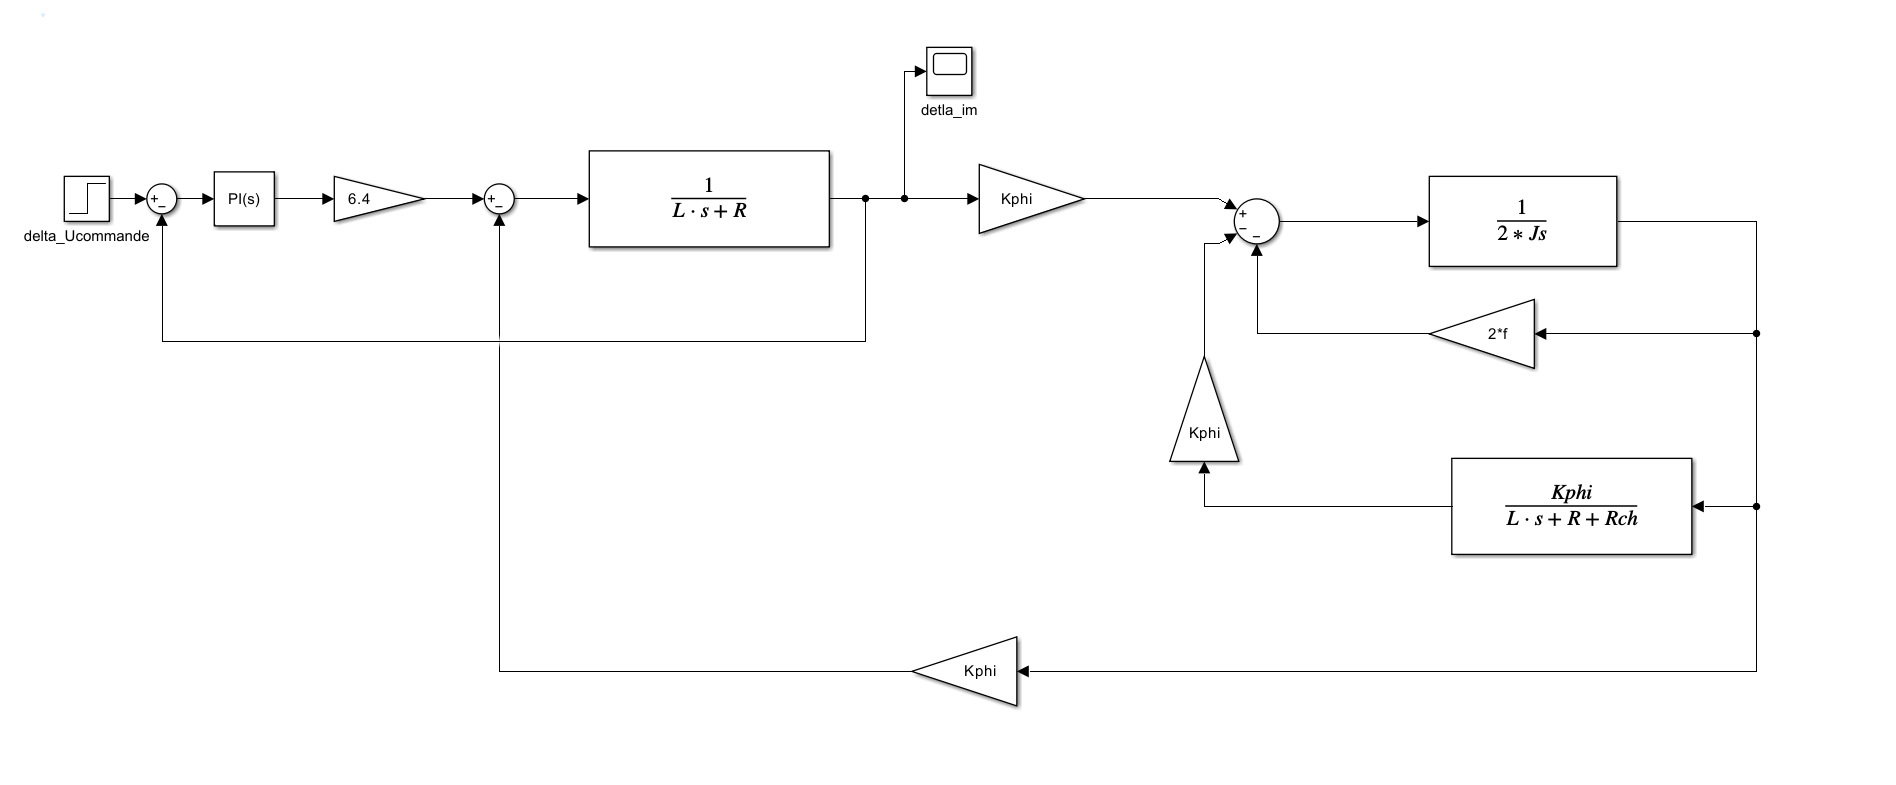
\includegraphics[width=1\textwidth]{images/boucle_de_courant/Simulink_boucle_de_courant.png}
    \caption{Schéma de l'asservissement en courant du moteur dans Simulink}
    \label{fig:asservissement_courant_simulink}
\end{figure}

% réponse indicielle de l'asservissement en courant Simulink
\begin{figure}[H]
    \centering
    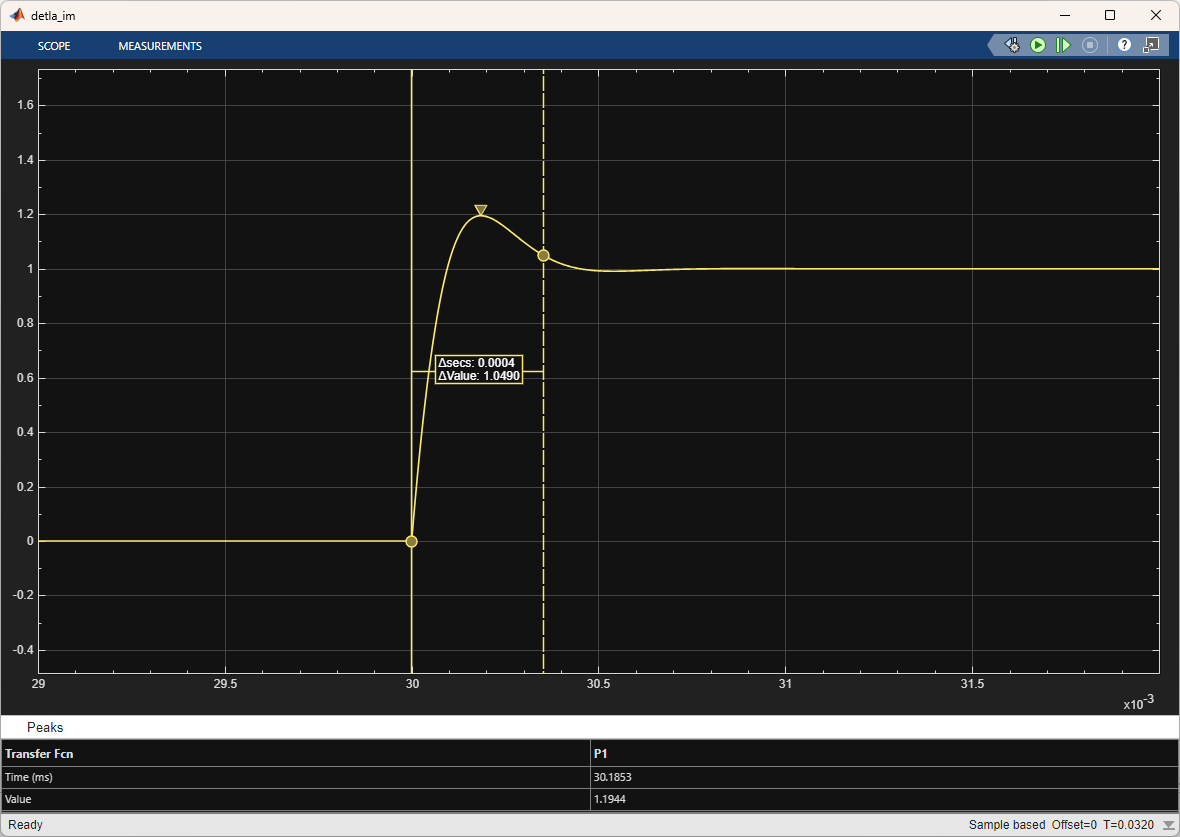
\includegraphics[width=1\textwidth]{images/boucle_de_courant/Simulink_reponse_indicielle_courant.png}
    \caption{Réponse indicielle de l'asservissement en courant du moteur dans Simulink}
    \label{fig:reponse_indicielle_courant_simulink}
\end{figure}

On constate que la réponse indicielle de l'asservissement en courant du moteur dans Simulink présente un dépassement d'environ 19\% et un temps de réponse de 0,35 ms. Ce qui respecte les spécifications du cahier des charges qui exige un dépassement maximal de 20\% et un temps de réponse maximal de 10 fois la prériode de la MLI soit 0,45 ms.

\subsubsection{Modélisation sur PSIM}

% image de l'asservissement en courant PSIM
\begin{figure}[H]
    \centering
    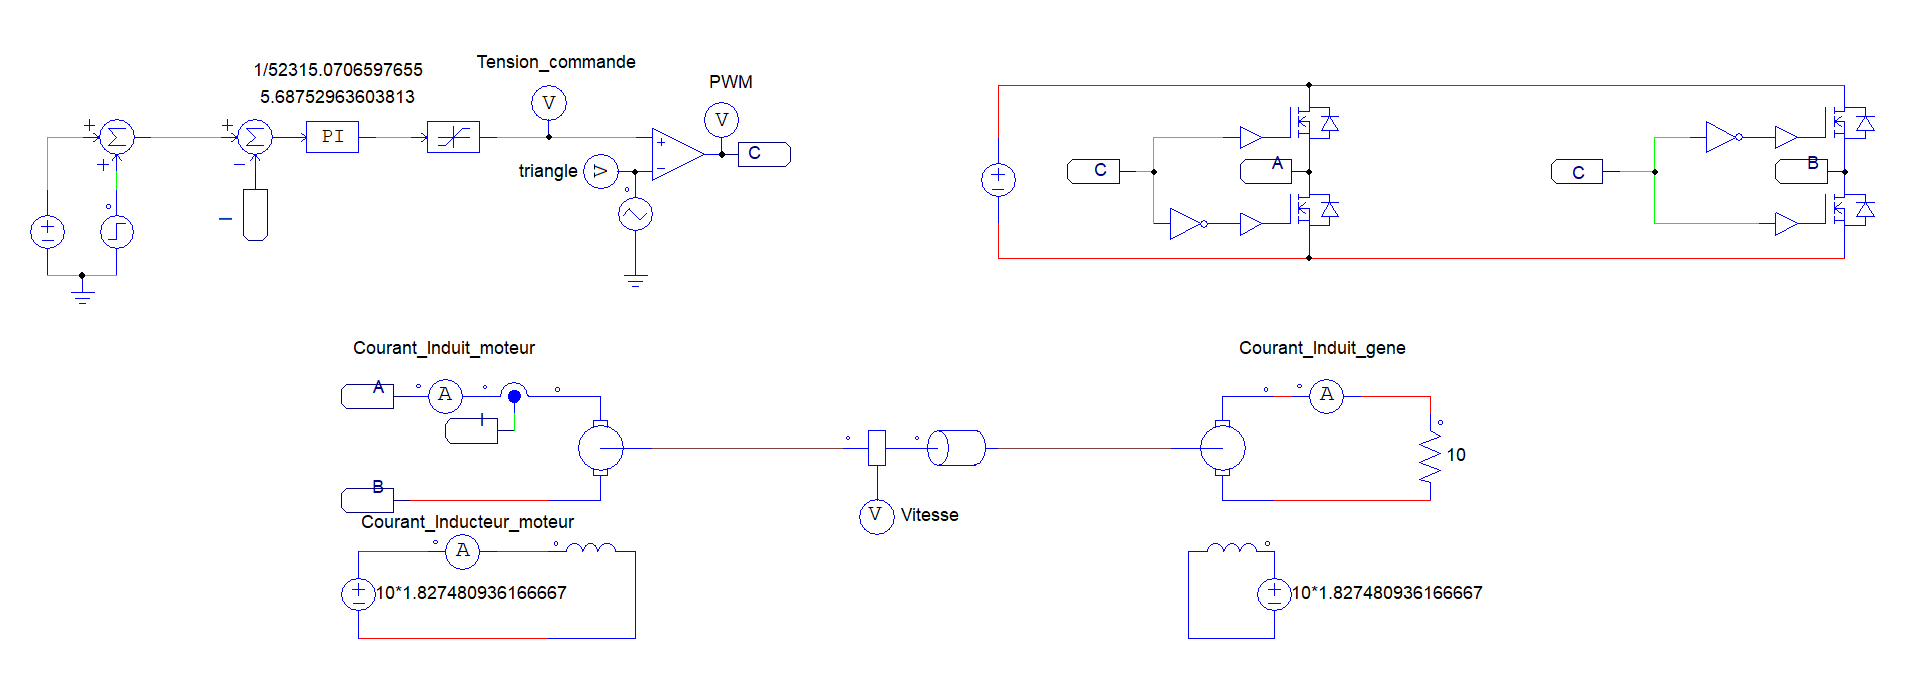
\includegraphics[width=1\textwidth]{images/boucle_de_courant/PSIM_boucle_de_courant.png}
    \caption{Schéma de l'asservissement en courant du moteur dans PSIM}
    \label{fig:asservissement_courant_psim}
\end{figure}
% réponse indicielle de l'asservissement en courant PSIM
\begin{figure}[H]
    \centering
    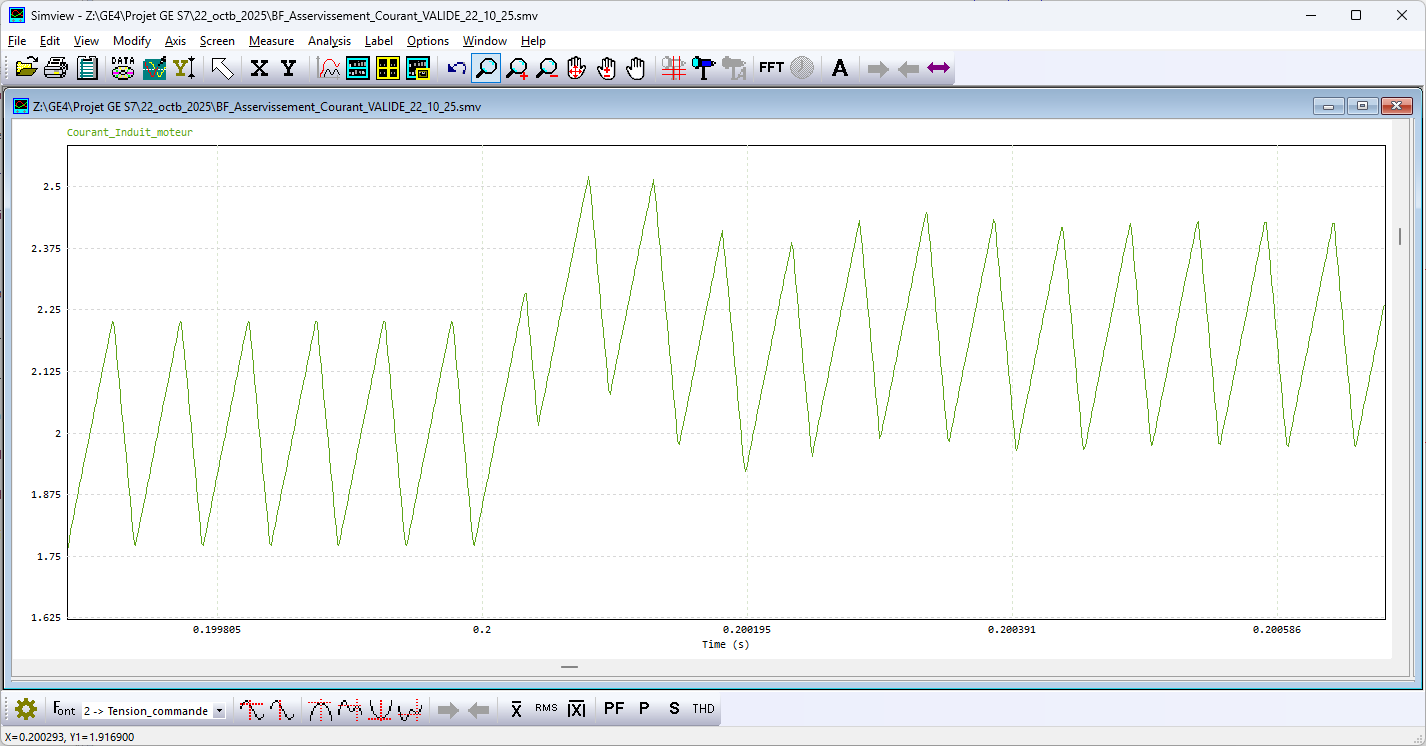
\includegraphics[width=1\textwidth]{images/boucle_de_courant/PSIM reponse indicielle courant BF.png}
    \caption{Réponse indicielle de l'asservissement en courant du moteur dans PSIM}
    \label{fig:reponse_indicielle_courant_psim}
\end{figure}

\subsubsection{Comparaison des résultats}

Dans cette section, nous allons comparer les résultats obtenus avec les deux outils de simulation, Simulink et PSIM.

% image de la comparaison des réponses
\begin{figure}[H]
    \centering
    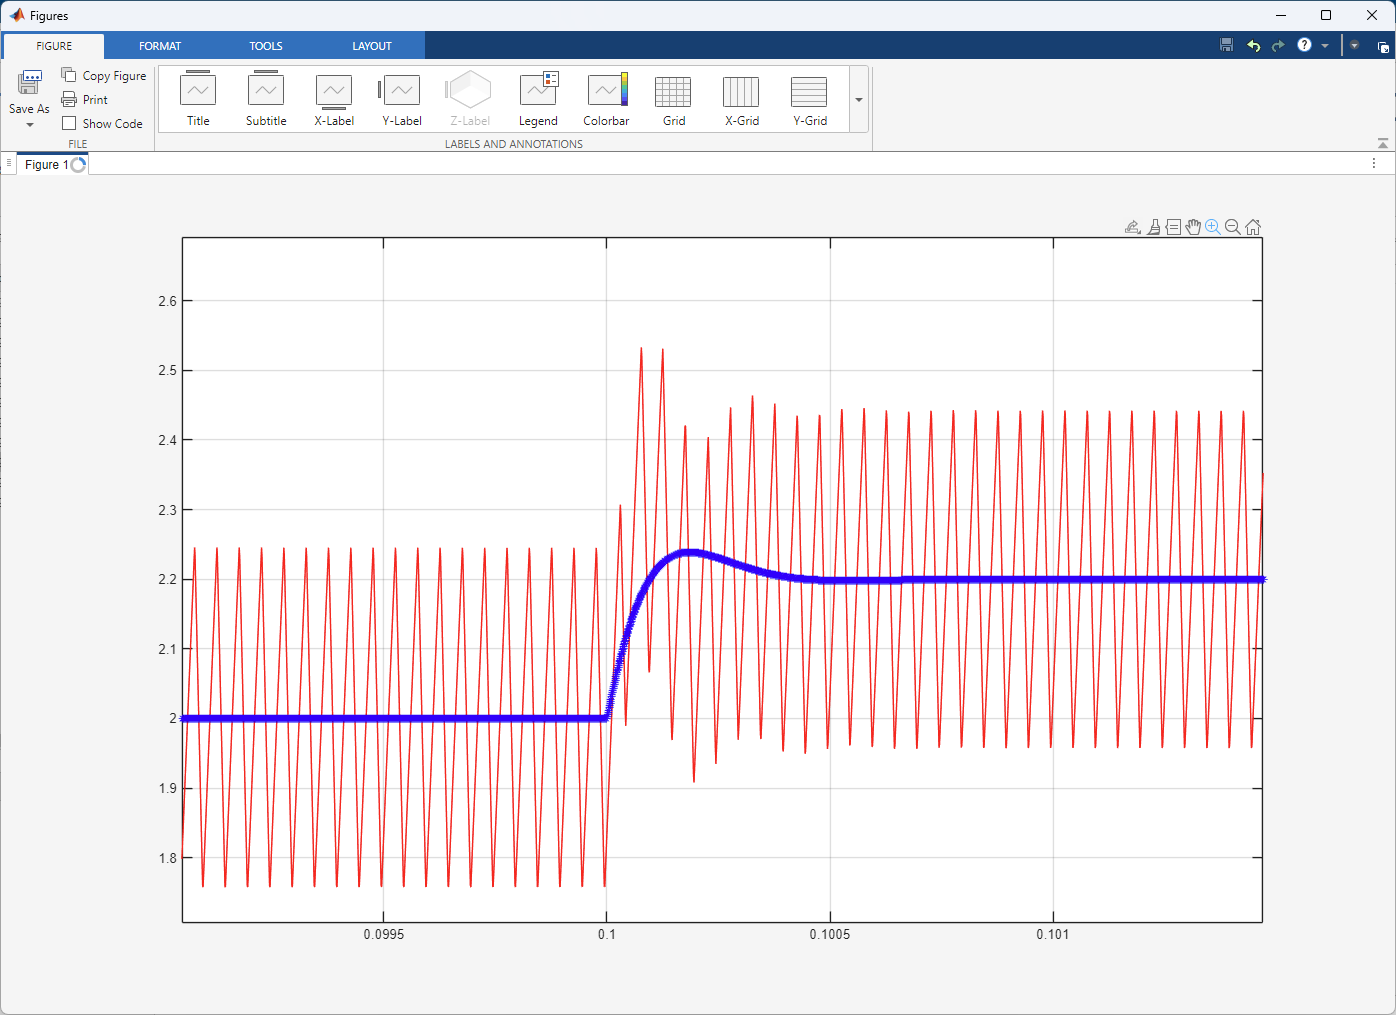
\includegraphics[width=1\textwidth]{images/boucle_de_courant/comparaison_reponse_indicielle_courant.png}
    \caption{Comparaison des réponses indicielle de l'asservissement en courant du moteur entre Simulink et PSIM}
    \label{fig:comparaison_reponse_indicielle_courant}
\end{figure}

\subsection{Asservissement en vitesse du moteur}

\subsubsection{Simulation sur Matlab/Simulink}
Nous commencons par la simulation de la vitesse du moteur en boucle ouverte sur Simulink. 

% réponse de l'asservissement en vitesse Simulink
\begin{figure}[H]
    \centering
    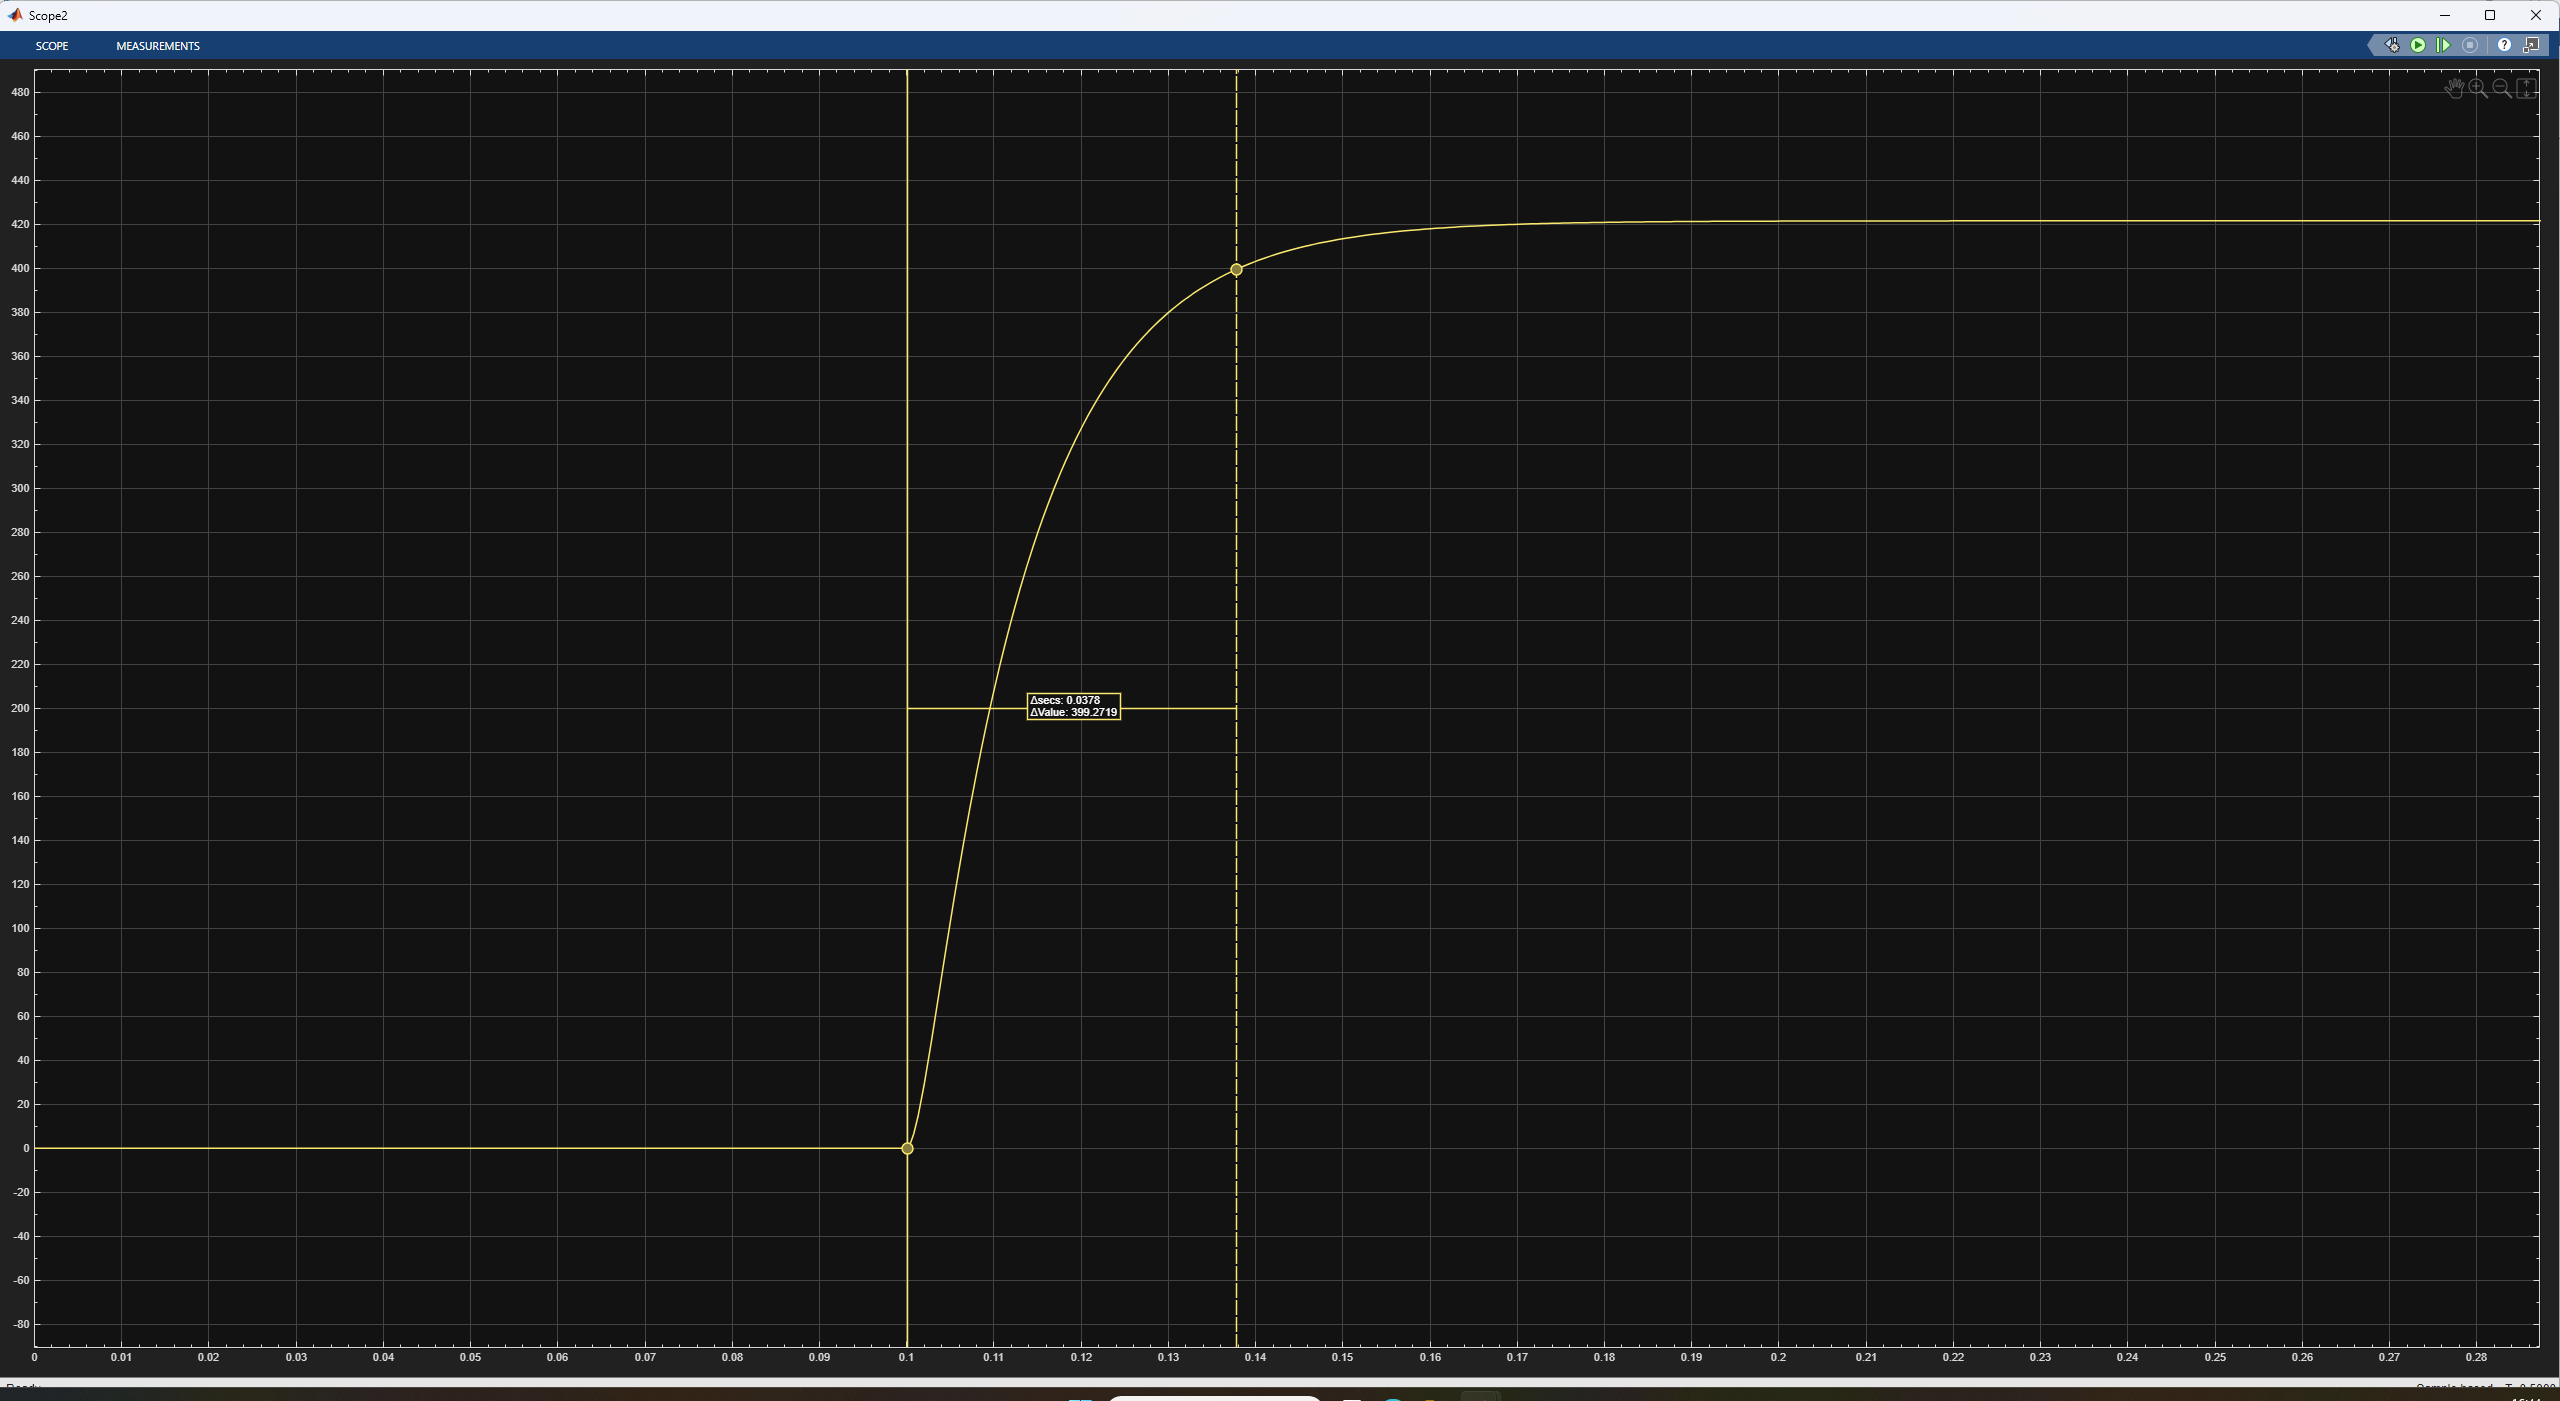
\includegraphics[width=1\textwidth]{images/asserv_de_vitesse_tachy/Vitesse_tr5_BO.png}
    \caption{Réponse de la vitesse du moteur en boucle ouverte dans Simulink}
    \label{fig:asservissement_vitesse_simulink}
\end{figure}
On releve un temps de réponse à 5\% en boucle ouverte pour la vitesse, sur Simulink : 37,8 ms

Nous cherchons ensuite à asservir la vitesse du moteur en boucle fermée avec un correcteur PI. Nous visons un temps de réponse à 5\% 3 fois plus rapide qu'en boucle ouverte soit 12,6 ms avec un dépassement maximal de 20\%.
\begin{figure}[H]
    \centering
    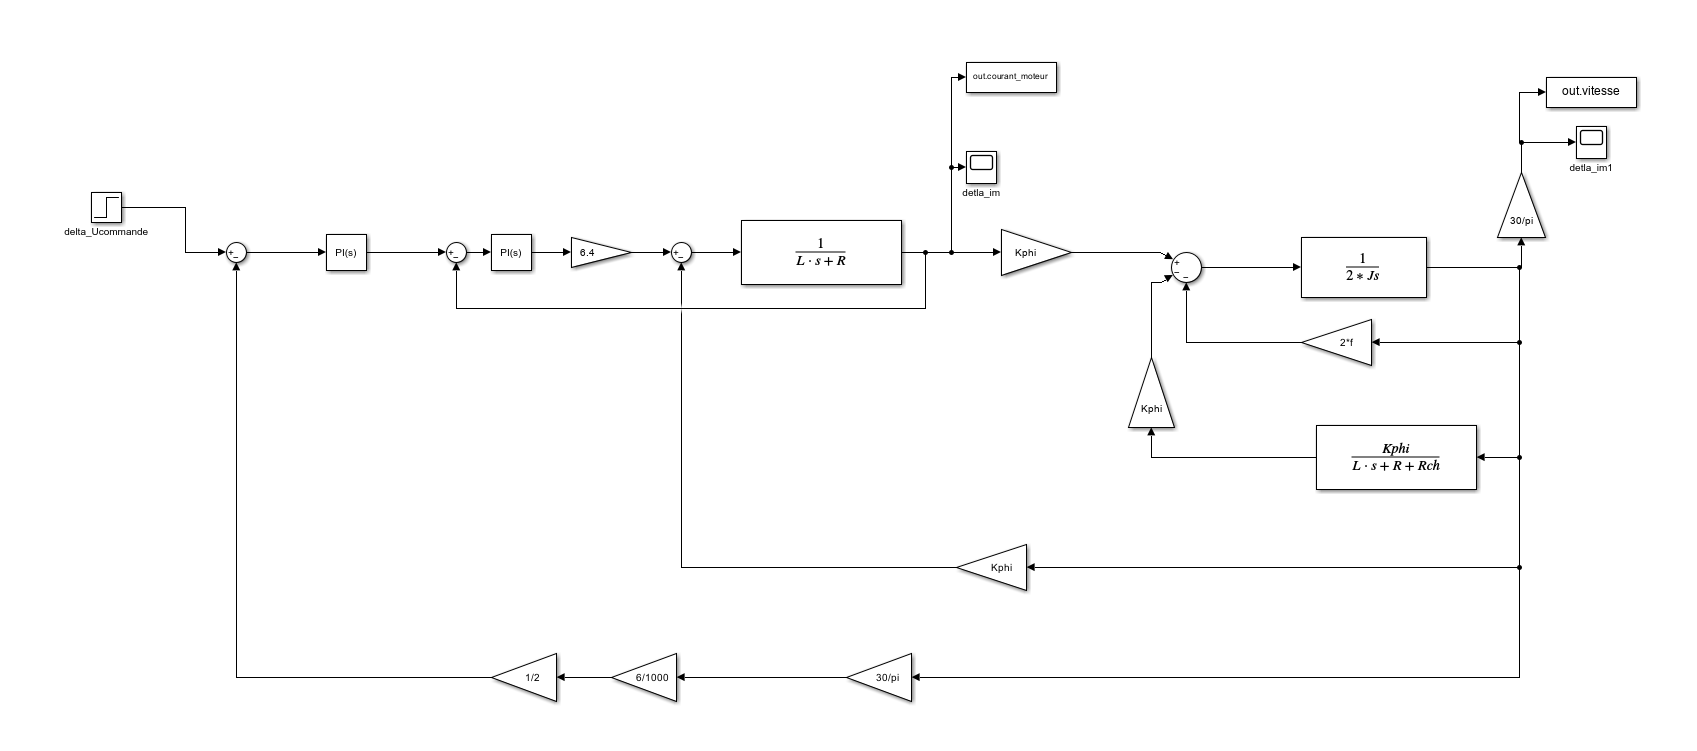
\includegraphics[width=1\textwidth]{images/asserv_de_vitesse_tachy/Simulink_boucle_de_courant_vitesse.png}
    \caption{Schéma de l'asservissement en vitesse du moteur dans Simulink}
    \label{fig:asservissement_vitesse_simulink_schema}
\end{figure}
A l'aide du PID Tuner de Simulink, nous obtenons les valeurs suivantes pour le correcteur PI :
\begin{itemize}
    \item $K_p = 37,3376029909659$
    \item $K_i = 14022,585396076$
\end{itemize}
% réponse de l'asservissement en vitesse Simulink
\begin{figure}[H]
    \centering
    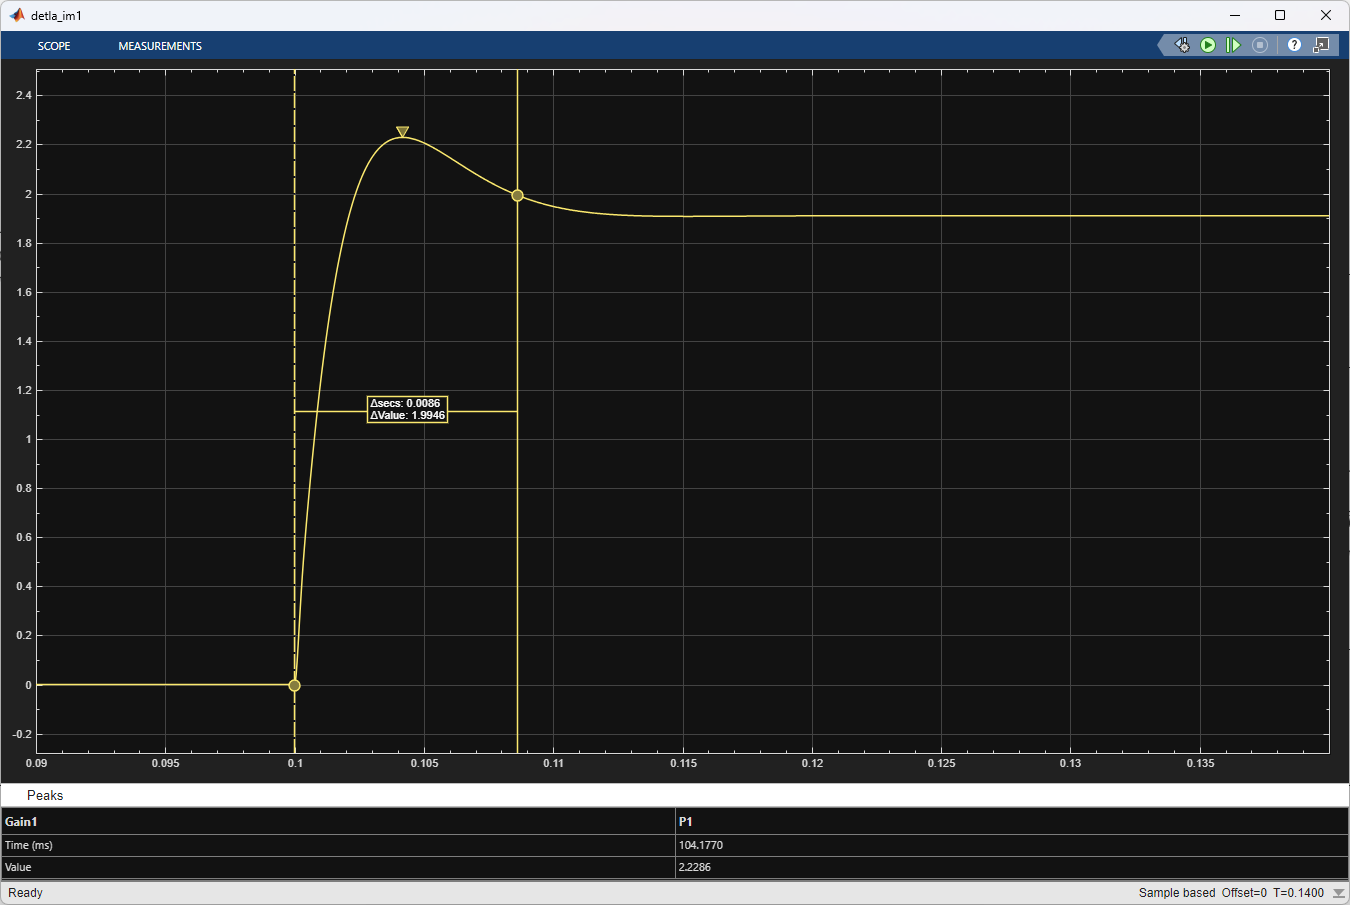
\includegraphics[width=1\textwidth]{images/asserv_de_vitesse_tachy/Vitesse_tr5_BF.png}
    \caption{Réponse de l'asservissement en vitesse du moteur dans Simulink}
    \label{fig:reponse_asservissement_vitesse_simulink}
\end{figure}
Nous relevons un temps de réponse à 5\% de 7,6 ms et un dépassement de 18,5\%, ce qui respecte les spécifications du cahier des charges.

\subsubsection{Simulation sur PSIM}

\subsubsection{Comparaison des résultats}
